\chapter{Performance tests}\label{C:Performance-Test}
In this chapter are shown the performance results for two tests carried out in a Raspberry Pi using the original implementation of IOSharp in C\# and running on Mono, and the C++ version which is a direct translation from the original using AlterNative.
\\
Theoretically, C++ has a major performance compared to C\# but this tests will be used to determine how much gains C++  over C\# in this case.
\\
To make the measures in this tests the Logic16 has been used. This is a channel analyser used to record, view, and measure digital signals.

\section{Compilation types}\label{S:PERF-comptypes}
When a compiler generates a binary from a source code normally tries to do some changes to optimize some attributes of the program. The most common requirement is to optimize the time taken to execute that program, another one is optimize the amount of memory required by the program. Also some optimizations can be used to make a program consume less power and this is interesting because nowadays the Internet of Things is in grown and many sensors have a small battery so reaching low-power consumption is great because it ensures a longest battery life or at least the sensor can operate more time. All of this optimizations are carried out by a sequence of optimizing transformations and algorithms applied using optimizing compilers.
\\
Normally compilers can generate programs optimized or non-optimized depending on how is configured the build system. If the compiler uses optimizations the compile time will growth but the program will be much more optimized than if the optimizations are not applied.
\begin{itemize}
  \item \textbf{Non-optimized or debug:} this mode is used by developers who want to debug applications in execution time. In this case the whole symbol information which is used by the debugger to stop at the break points (designated instructions) is attached to the generated assembly. For example the \verb!*.pdb! files from Visual Studio are created by the compiler and have the information to debug the created assembly. On the other hand, the debug mode will not allow some optimizations because are incompatible with the debugging functionality.
  \item \textbf{Optimized or release:} this mode is used to generate an optimized assembly to run or perform much faster than the debug one. In this case the compiler performs different transformations to the original code, for example two typical optimizations that cannot be applied to a debug build are:
  \begin{itemize}
  	\item \textbf{Loop unrolling:} the compiler analyses how many times the loop is executed and then it copies the inner code the same number of times. This helps avoiding the maintenance of the loop variables.
  	\item \textbf{Inlining:} the compiler places the method on the place of the call avoiding the stack overhead produced by a method's call.
  	\begin{lstlisting}[language=C++, caption={Inline example}]
inline int Max(int x, int y)
{
   return (x > y)? x : y;
}
int main( )
{
   int a = 100;
   int b = 1010;
   cout << "Max (a, b): " << Max(a, b) << endl;
   return 0;
}

/* The Max(int, int) function is inlined to the main Max call in the following way:*/
int main( )
{
   int a = 100;
   int b = 1010;
   cout << "Max (a,b): " << (a>b)? a : b << endl;
   return 0;
}
\end{lstlisting}
  \end{itemize}
\end{itemize}

\section{GPIO}\label{SS:IOEx-GPIO}
GPIO test consists on how much time takes the board to perform a certain number of iterations changing an output port between the high and low states. Two channels are used in this test, the first one will activate the Logic16 to start sniffing the second channel which will be the one that performs the changes. 
\\
\\
The following code shows the test using the C\# implementation. This is the minimum test to analyse the performance of Mono and C++ when I/O is involved using the original IOSharp and its translation. In this case, it will be measured the whole time that the system takes to change the state of an output port on a certain number of iterations.
\begin{lstlisting}[language=CSharp, caption={GPIO Performance test in C\#}]
using System;
using System.Collections.Generic;
using System.Linq;
using System.Text;
using Microsoft.SPOT.Hardware;
using IOSharp.NETMF.RaspberryPi.Hardware;
using System.Threading;

namespace raspberrypi
{
    class Program
    {
        public static void Main()
        {
            Debug.Print("START");
            OutputPort bar = new OutputPort(Pins.V2_GPIO17, false);
            bar.Write(false);
            bool foo = false;
            OutputPort o = new OutputPort(Pins.V2_GPIO11, false);

            bar.Write(true);
            for (int i = 0; i < 10000; i++)
            {
                foo = !foo;
                o.Write(foo);
            }
            bar.Write(false);
            Debug.Print("END");
        }
    }
}
\end{lstlisting}
And the following one corresponds with the C++ translation.
\begin{lstlisting}[language=C++, caption={GPIO Performance translated to C++}]
#include "Program.h"
namespace raspberrypi {

	void Program::Main(){
		Program* p = new Program();
		p->Run();
	}

	void Program::Run(){
		Debug::Print(new String("START"));
		OutputPort* bar = new OutputPort(Cpu::Pin::GPIO_Pin17, false);
	
		bar->Write(false);
		bool foo = false;
		OutputPort* o = new OutputPort(Cpu::Pin::GPIO_Pin11, false);
		bar->Write(true);
		for (int i = 0; i < 200; i += 1) {
			Debug::Print(new String(i));
			foo = !foo;
			o->Write(foo);
		}
		bar->Write(false);
		Debug::Print(new String("END"));
	}
}
\end{lstlisting}

This test has been executed varying the number of iterations between 200 and 10000. Each iteration swaps the port state between high and low. Apart from this iteration increase, the assembly is compiled using the compiling modes explained above (debug and release modes).

\subsection{200 Iterations}\label{SS:200-iterations}
The result produced by Mono with the binary compiled with optimizations shows an irregular pattern consisting of two small pulses followed by a wide pulse and then two small pulses followed by wide gap. In the figure \ref{fig:gpio-200it-csharp} this pattern is coloured in blue and as it can be seen it is regularly repeated across all the iterations. The wide pulses and gaps are supposed to be caused by the garbage collector and the thread round-robin that Mono does.
\\
The small pulses are around 1 ms and the wide gaps/pulses are 2 ms long. Each block is repeated every 10 ms.
\begin{figure}[H]\begin{center}
 \centering
  \captionsetup{justification=centering}
  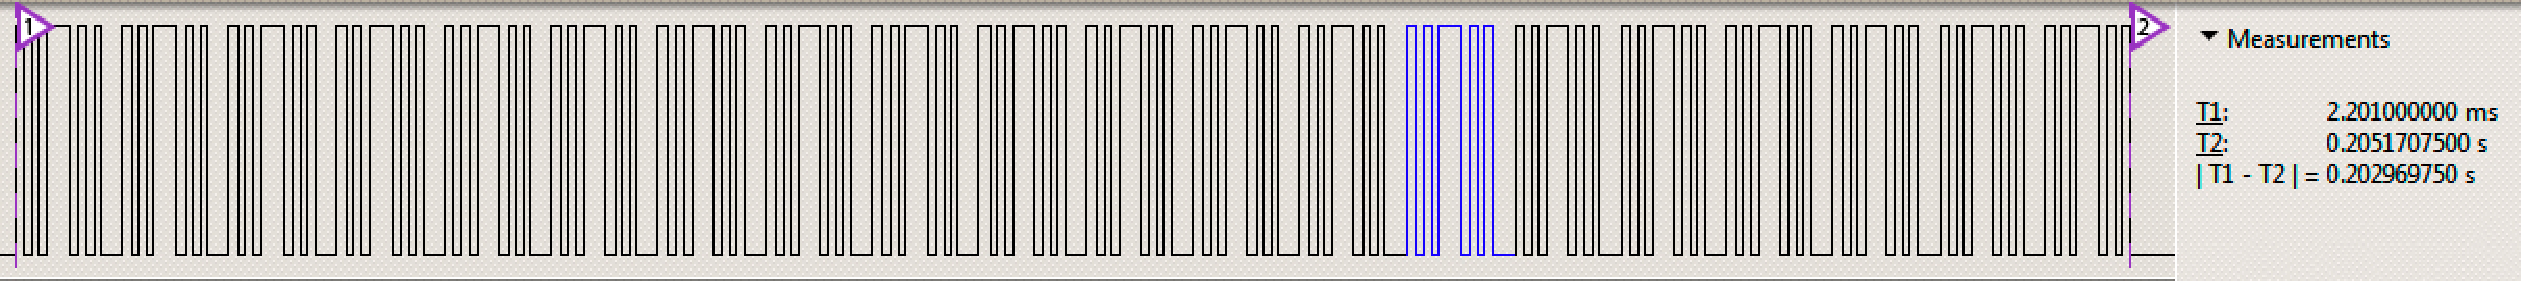
\includegraphics[scale=0.35]{pictures/performance-tests/GPIO/200/csharp2}
  \caption{200 Iterations using C\# with optimizations\label{fig:gpio-200it-csharp}}
\end{center}\end{figure}
The figure \ref{fig:gpio-200it-csharp} represents this 200 changes in the output state. The required time to make this iterations is the elapsed time between the marker 1 and the marker 2. The Raspberry Pi with Mono needs 202 ms in order to do all the iterations.
\\
\\
After testing the performance in Mono it was time to try out the code generated by AlterNative which is also compiled in release mode. The resulting test is shown and explained below.
\begin{figure}[H]\begin{center}
 \centering
  \captionsetup{justification=centering}
  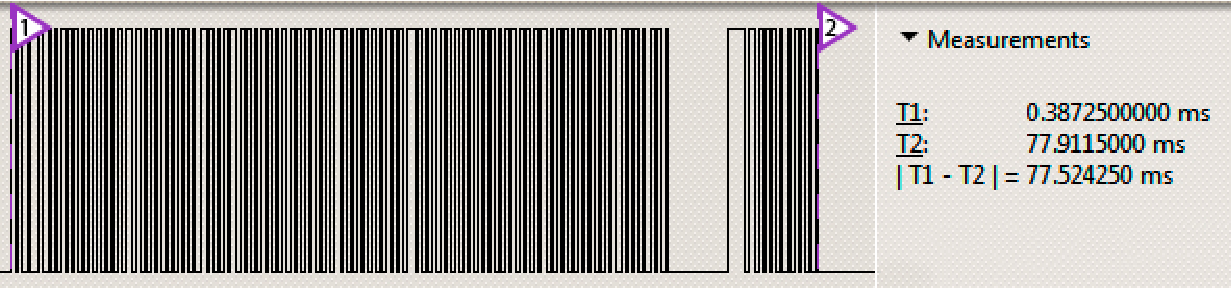
\includegraphics[scale=0.35]{pictures/performance-tests/GPIO/200/cxx}
  \caption{200 Iterations using C++ with optimizations \label{fig:gpio-200it-cxx}}
\end{center}\end{figure}
This above image uses the same scale as the figure \ref{fig:gpio-200it-csharp} shows, so the magnitude of the elapsed time can be compared.
\\
\\
In the case of C++ test, it can be observed that the pulses are much more regular than the Mono test, but at certain point around the pulse 89 a big gap is observed probably due to the lack of a garbage collector (AlterNative programs currently do not have a working garbage collector implemented). It is relevant to remark that C++ needs only 77 ms to perform the same test, and each pulse is 0.43 ms on average.
\\
\\
After doing some tests on debug and release mode in both languages a graphic could be sketched, the performance in 200 iterations on Mono using both compile types was the practically the same, it took around 200 ms to complete all the test, however in C++ the time varies a bit depending on the compilation type, without using optimizations it takes 100 ms but when optimization is applied the time decreases to 78 ms.
\\
From the figure \ref{fig:gpio-graph-200} can be concluded that the C++ version is a 62\% faster than the Mono one.
\begin{figure}[H]\begin{center}
 \centering
  \captionsetup{justification=centering}
  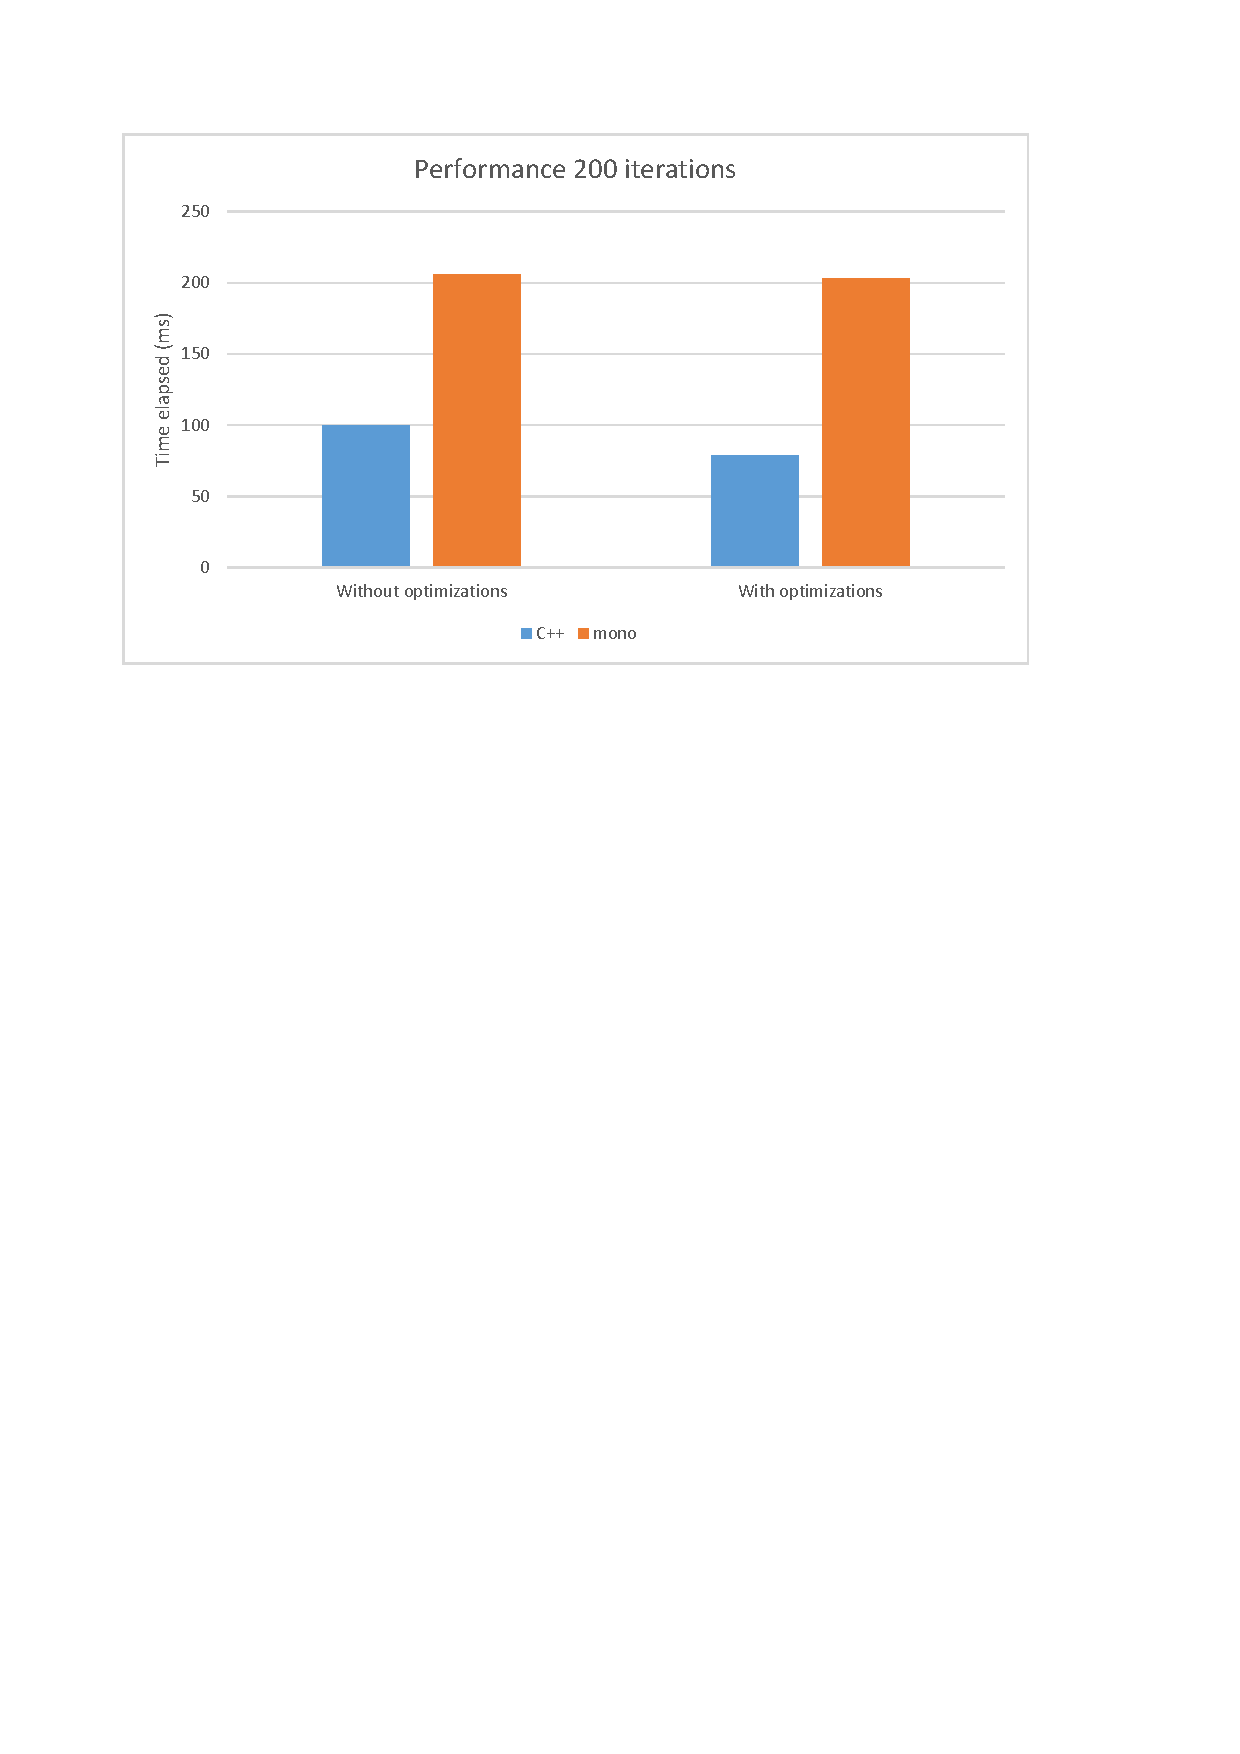
\includegraphics[scale=0.9,page=1]{pictures/performance-tests/GPIO/graphs}
  \caption{Graph showing the elapsed time for the 200 iteration test. Blue is for C++ while orange is C\#. On the left is represented the non-optimized compilations and on the right the optimized ones\label{fig:gpio-graph-200}}
\end{center}\end{figure}

\subsection{10K Iterations}\label{SS:10K-iterations}
After testing the 200 iterations another one was done, but increasing the number of iterations to 10000 or in a factor of fifty, in this magnitude the compiler optimizations should be visible enough to observe some kind of improvement on the different compilation and language types.
\\
In the figure \ref{fig:gpio-10kit-csharp+cpp} is represented the elapsed time for 10k iterations, the block on the left is the Mono version and lasts 10 seconds while the second one is the C++ version and the iterations are done in approximately 3 seconds being approximately three times faster.
\begin{figure}[H]\begin{center}
 \centering
  \captionsetup{justification=centering}
  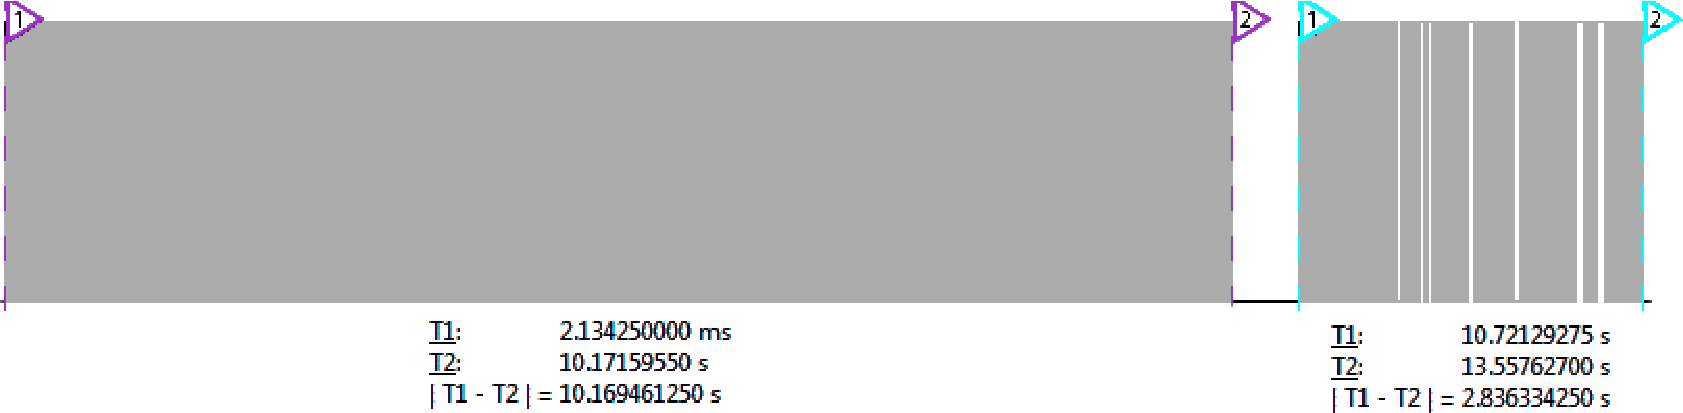
\includegraphics[width=1\textwidth]{pictures/performance-tests/GPIO/10k/cxx+csharp}
  \caption{10k Iterations using C\# with optimizations \label{fig:gpio-10kit-csharp+cpp}}
\end{center}\end{figure}
As it was done in the previous test a graph has been done comparing the different languages and compilation types.
\begin{figure}[H]\begin{center}
 \centering
  \captionsetup{justification=centering}
  \includegraphics[scale=0.9,page=2]{pictures/performance-tests/GPIO/graphs}
  \caption{Graph showing the elapsed time for the 10k iteration test. Blue is for C++ while orange is C\#. On the left is represented the non-optimized compilations and on the right the optimized ones\label{fig:gpio-graph-10k}}
\end{center}\end{figure}
At this number of iterations the C++ performs much better than C\# and also is possible to see an improvement between the debug and release versions of C++ being the optimized version 741 ms faster than the non-optimized one.

\section{Interruptions}\label{S:Performance-Interruptions}
It was observed that in HomeSense the response time in the sensor events was poor, probably because of the time that Mono takes between the interruption detection and the interception response. To analyse the elapsed time between the trigger and the response the example will be polling events from a pin, when an event occurs another pin  will be used in output mode with an active high state.
\\
Like the previous test, the C++ code has been generated using AlterNative so it also will be used to test some special functionalities like the delegates or the timer. The program will start and create a delegate which will be the called function when an interrupt occurs.
\\
In the figure \ref{fig:interrupt-csharp} is shown the triggering of the interruption (the top channel with the falling edge), after 1.326 ms the second channel is activated in state high which represents the interruption response.
\begin{figure}[H]\begin{center}
 \centering
  \captionsetup{justification=centering}
  
\includegraphics[scale=0.65]{pictures/performance-tests/Interruptions/csharp}
  \caption{Response time of an interruption in C\# and Mono\label{fig:interrupt-csharp}}
\end{center}\end{figure}
Then the same test is performed using the C++ version. The result is pretty good because the interruption is attended only 0.879 ms after the triggering. This implies that C++ is 447 $\mu$s faster than C\#.
\begin{figure}[H]\begin{center}
 \centering
  \captionsetup{justification=centering}
  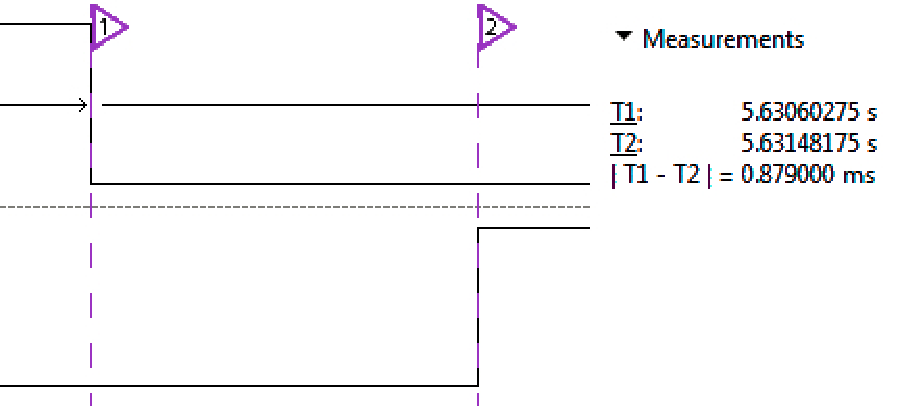
\includegraphics[scale=0.65]{pictures/performance-tests/Interruptions/cxx}
  \caption{Response time of an interruption in C++\label{fig:interrupt-cxx}}
\end{center}\end{figure}
It is important to remark that the interruptions in operating systems cannot be considered real-time interruptions, this implies that sometimes an event is attended at a certain time but in another moment the time required can be much more different due to the non real-time kernel that usually Linux uses. If a hard real-time is needed it is recommended to use other platforms like FreeRTOS which is intended to do tasks that require controlled response times.